\begin{newpage}
  \section{Discover}
  \label{sec:discover}
    In der Discover Phase soll der Blickwinkel möglichst weit geöffnet werden. 
    Dafür erfolgte eine weitreichende Recherche zu relevanten Themenbereichen wie Live Visualisierung, Visualisierung von öffentlichem Nahverkehr sowie Tools zum Erstellen von Karten (Abbildung \ref{fig:viz_overview}). Darüber hinaus wurden mögliche Datenformate auf ihre Vor- und Nachteile untersucht. Die wichtigste Frage stellt sich allerdings hinsichtlich der möglichen Zielgruppe, die von einer Visualisierung von Echtzeitdaten profitieren könnte. Nach dieser müssen sich schließlich die zu implementierenden Funktionen und Features richten. Die wichtigsten Überlegungen und Rechercheergebnisse zu diesen Aspekten sollen in den folgenden Abschnitten beschrieben werden. 

    \subsection{Related Work}
\label{sub:related_work}
  Es existieren mehrere Publikationen, welche für diese Arbeit Relevanz haben oder die für dieses Thema wertvolle Informationen bereitgestellt haben. Die wichtigsten werden in diesem Abschnitt vorgestellt.\\

  Einen ersten guten Überblick zum momentanen Stand von Transportvisualisierungen bietet das Paper \textit{"`Visualizing Public Transport Systems: State-of-the-Art and Future Challenges"'}\parencite{marchi} von Massimo De Marchi. In seiner Arbeit wird dargelegt, welche visuellen Lösung bereits bestehen und welche stärken / schwächen sie haben. Dabei wird auf Zwei unterschiedliche Benutzertypen eingegangen. Namentlich als "`Traveler"' und "`Transportation Researcher"' genannt. Er beschreibt dabei welche verschiedenen Eigenschaften die jeweilige Nutzerrolle besitzt und welche Bedürfnisse diese haben. Diese Frage \textit{"`Wer soll die interaktive Karte am ende benutzen?"'} ist auch bei der Erstellung dieser Arbeit von entscheidender Bedeutung gewesen. Je nach Typ bedarf es einem anderen Schwerpunkt gerecht zu werden. In dieser Arbeit sollen vor allem diejenigen einen Nutzen daraus ziehen können, die\\

  \parencite{mbtaviz} beschreibt sehr gut die Vorgehensweise und verwendeten Technologien für die Umsetzung der Visualisierung von \textit{"`An interactive exploration of Boston's subway system"'}\footnote{\url{http://mbtaviz.github.io/}}. Es werden dabei sowohl die verwendeten Tools beschrieben als auch Mockups gezeigt die eindrücke in den Arbeitsprozess gewähren. Die resultierenden Visualisierungen und deren Detailgrad sind sehr Eindrucksvoll und lassen einen tiefen Einblick in das Verkehrsnetz zu.\\

  Eine weitere wertvolle Quelle ist die Arbeit von Patrick Brosi \textit{"`Real-Time Movement Visualization of Public Transit Data"'}\parencite{brosi}. Brosi stellt dabei die Entwicklung von Travic vor, der bereits eingangs\footnote{siehe Kapitel \ref{travic}} erwähnt wurde. Seine Arbeit zeigt einen Lösungsweg für die Visualisierung von Tausenden Fahrzeugen auf einer interaktiven Karte. Interessant sind dabei die diskutierten Vor- und Nachteile von verschiedenen Lösungsansätzen.
  Während seine Arbeit keine Datenbank verwendet, sondern alle Daten in den RAM-Speicher des Servers läd, um schnelle Zugriffszeiten zu erreichen, soll in unserer Arbeit eine Postgresql Datenbank zum Einsatz kommen. 
  Auch hat unsere Arbeit nicht den Anspruch eine weltweite Live Karte zur Verfügung zu stellen, sondern fokussiert sich lediglich auf den Raum Stuttgart unter Verwendung eines GTFS Feeds des Verkehrsverbundes Stuttgart-VVS. 
  Der Kern der Arbeit beschäftigt sich tiefer mit dem finden von neuen Visualisierungsansätzen und UI-Komponenten. Es steht also nicht die Entwicklung eines fertigen Produkts im Vordergrund, sondern viel mehr darum, wie Nutzern auf visuellem Weg Informationen auf interessante Weise präsentieren werden können.

% sec:related_work (end)

    \subsection{Visualisierungsmöglichkeiten und Zielgruppe}
\label{sub:visualisierungsmöglichkeiten_und_zielgruppe}
  \begin{figure}[ht]
    \begin{center}
      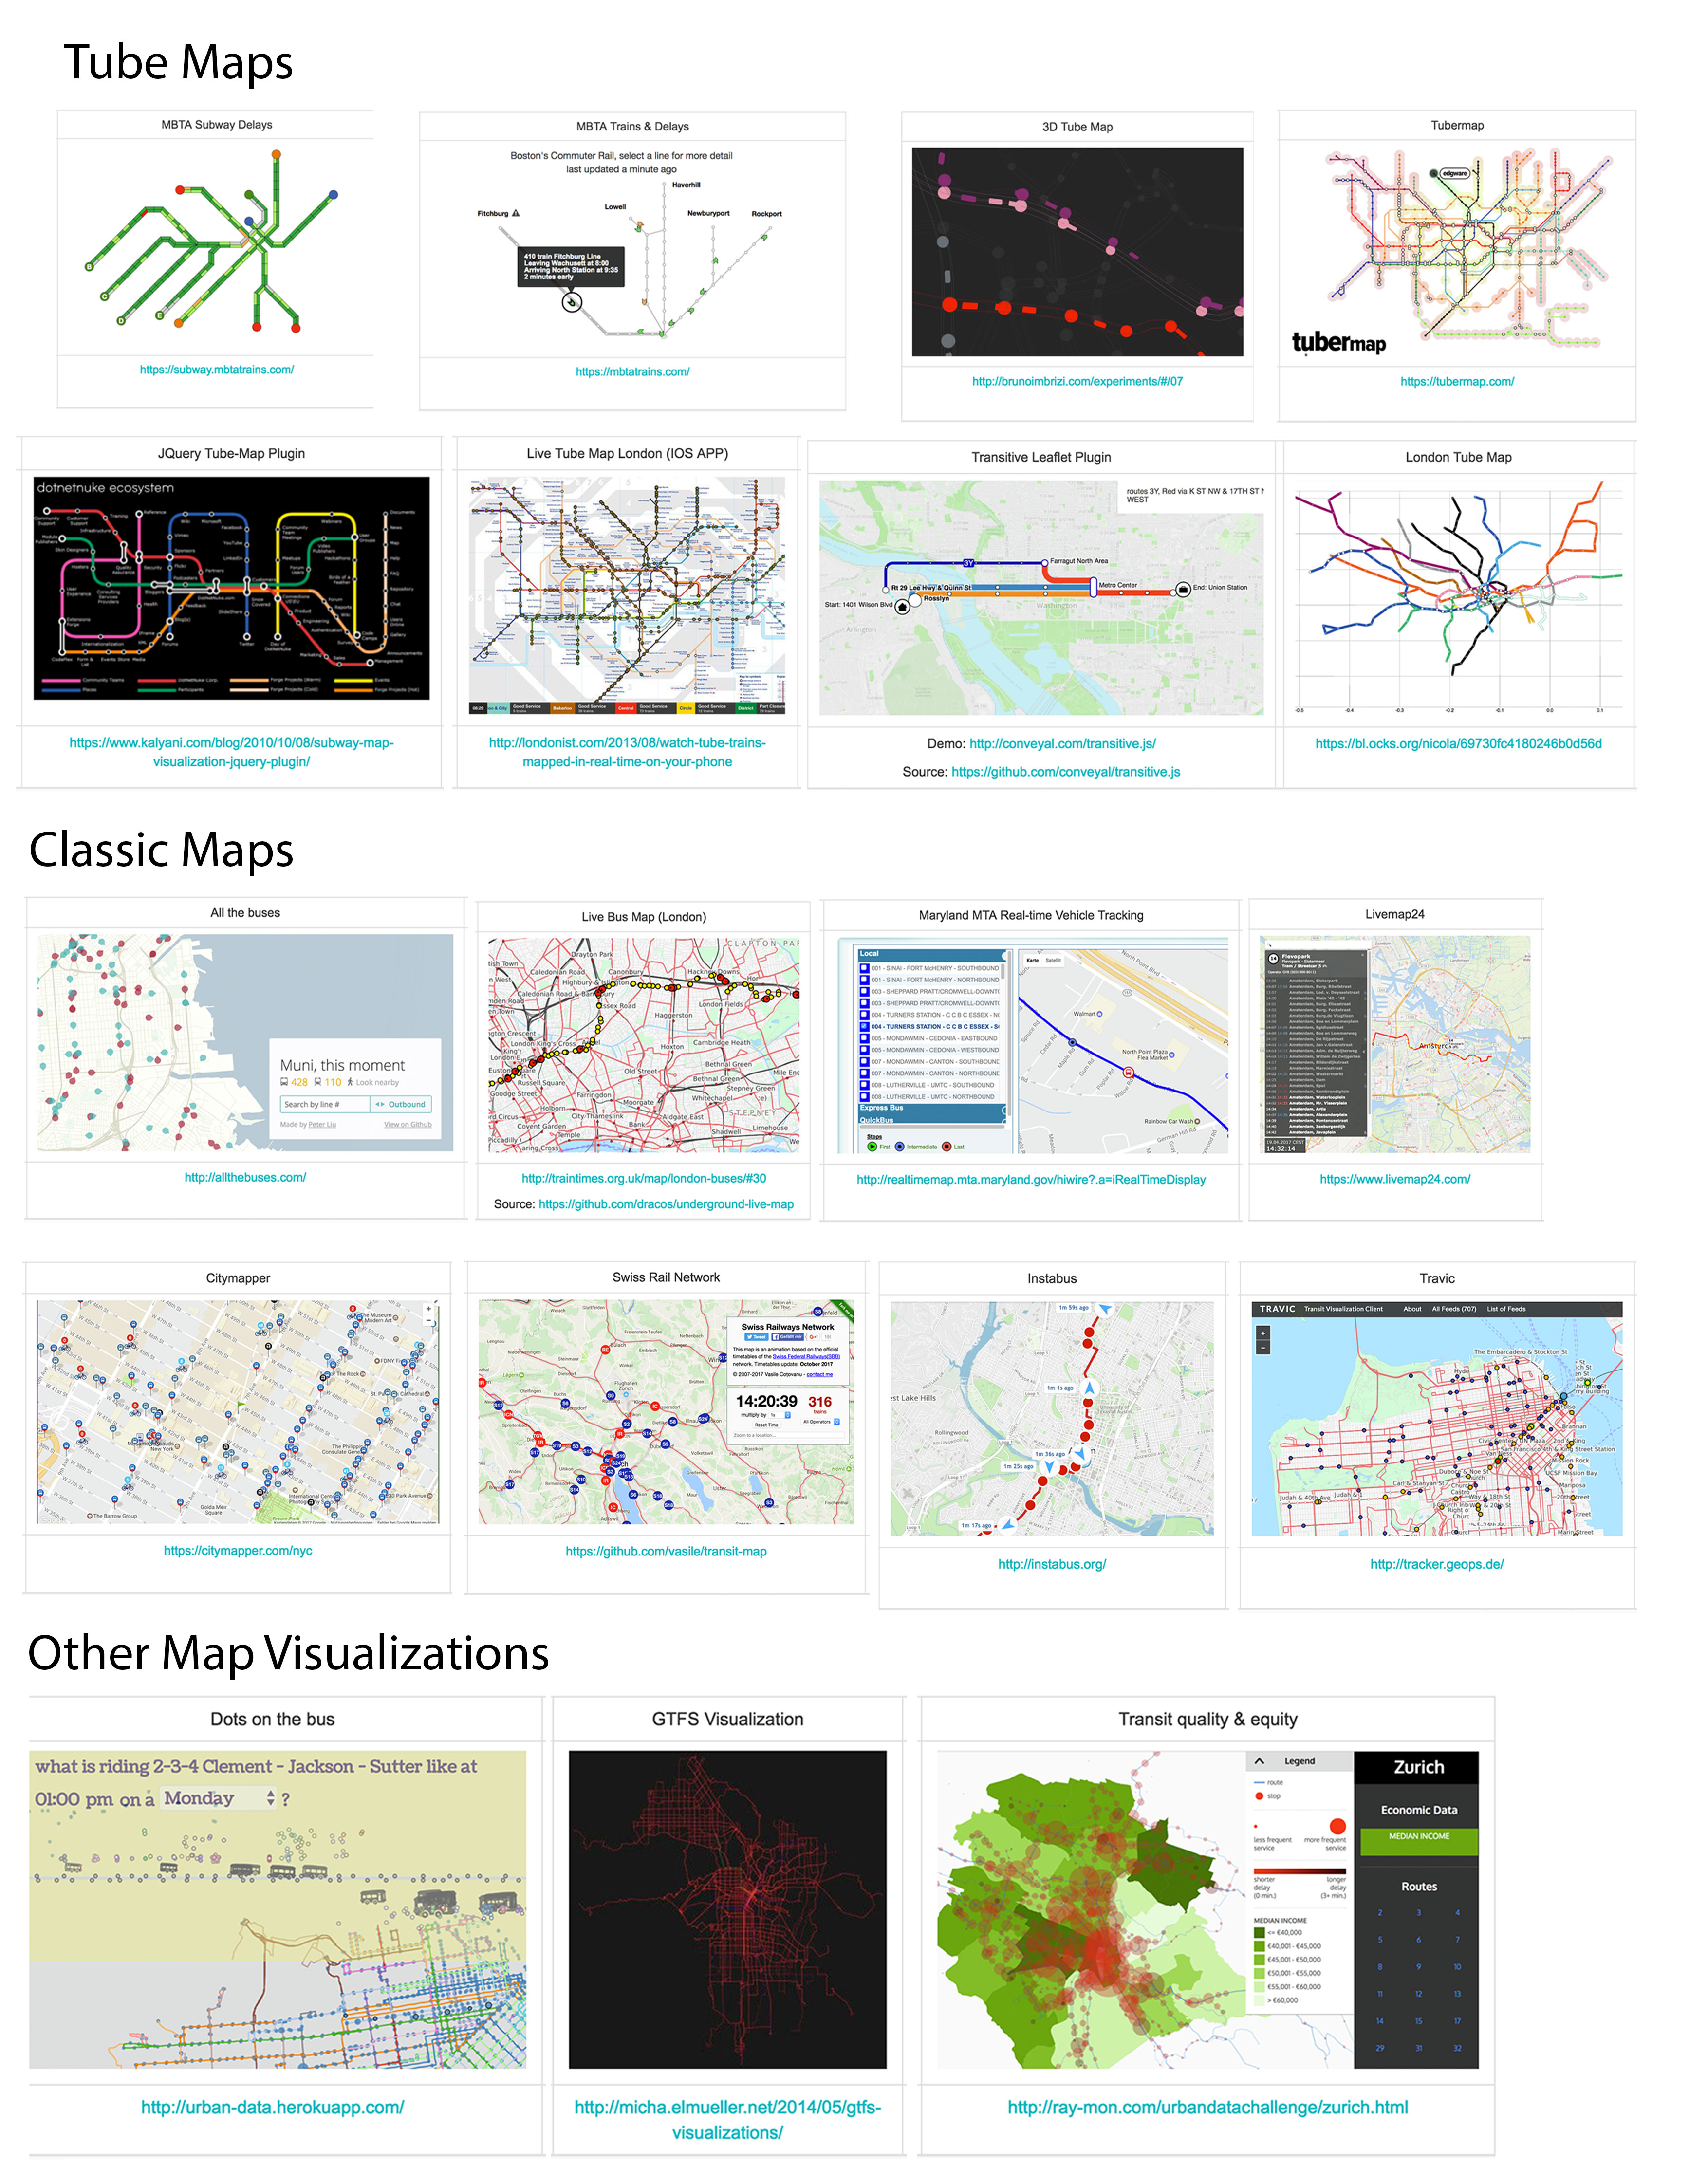
\includegraphics[width=0.8\textwidth]{viz_overview}
      \caption{Überblick über bestehende Tools und Visualisierungen}
      \label{fig:viz_overview}
    \end{center}
  \end{figure}

  Das gesammelte Material wurde in einer 2x2 Matrix (Abbildung \ref{fig:2x2_matrix}) in die Unterkategorien "`Live Map, Künstlerische Visualisierung, Plugin / Software / Tool, Tube-Map"' eingeordnet um einen sortierten Gesamtüberblick zu bekommen. 

  \begin{figure}[htbp]
    \begin{center}
      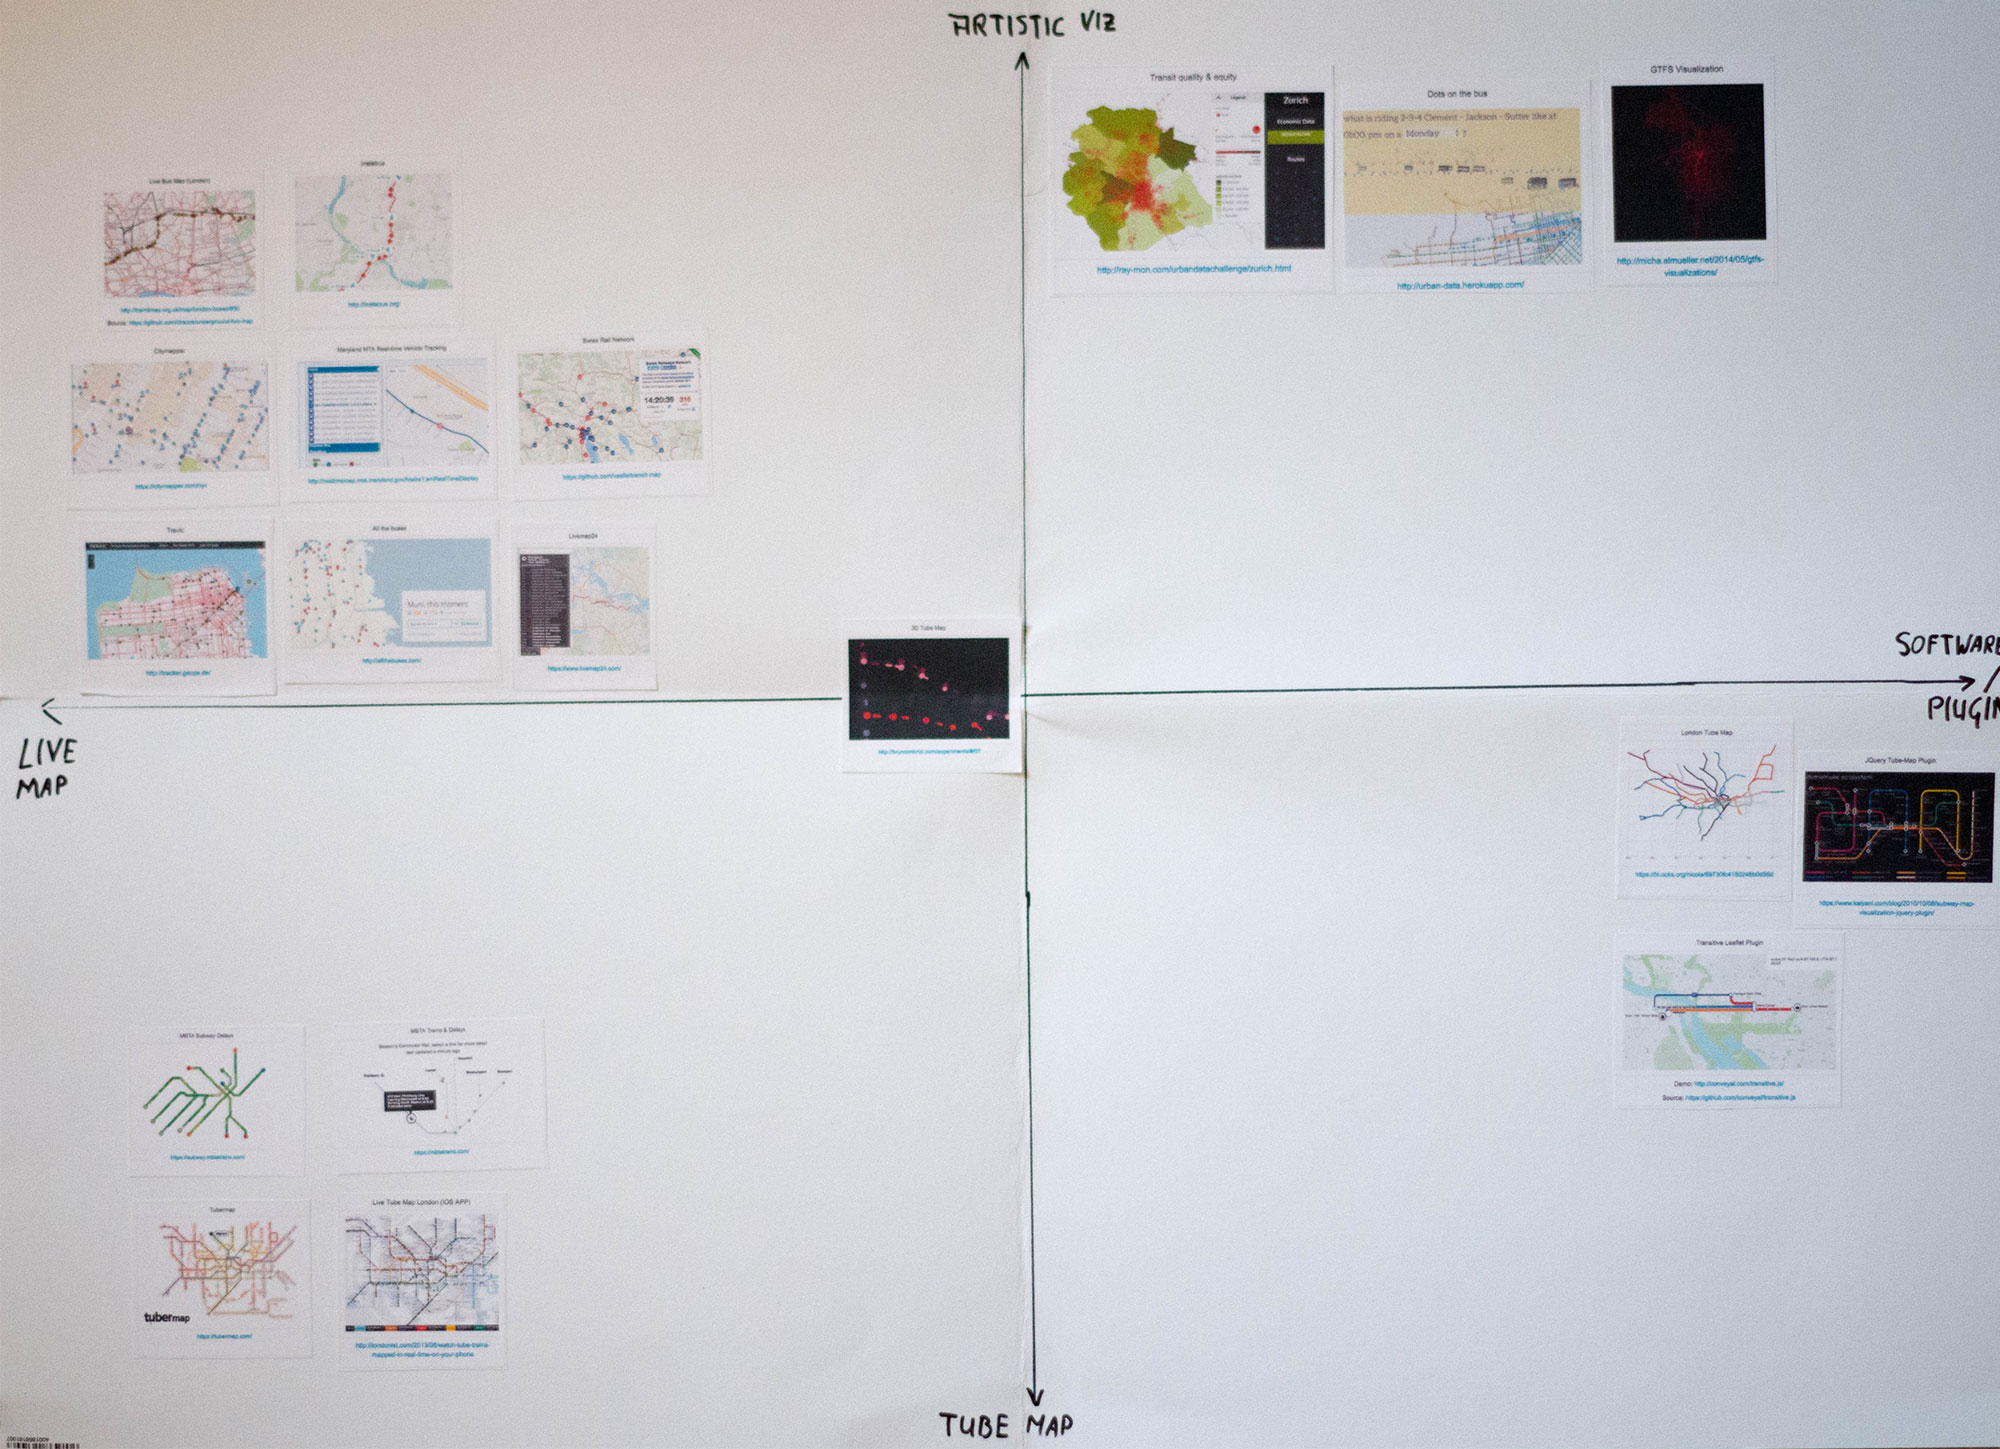
\includegraphics[width=0.5\textwidth]{2x2_matrix}
      \caption{2x2 Matrik Methode auf DIN A2}
      \label{fig:2x2_matrix}
    \end{center}
  \end{figure}

  Durch diese Ansicht wurde die Erkenntnis gewonnen, dass es schon viele Live Visualisierungen auf interaktiven Karten gibt, aber nur sehr wenig so genannten Tube-Maps. Auch sind bereits verschiedenste Tools zum generieren von GTFS basierten Visualisierungen vorhanden. Eine sehr ausführliche, aber bei weitem nicht vollständige, Liste über das Thema "`Transit"' wurde auf Github von der Community zusammengetragen \url{https://github.com/luqmaan/awesome-transit}.
% subsection visualisierungsmöglichkeiten_und_zielgruppe (end)
    \subsection{Mögliche Datengrundlage und Format}
\label{sub:mögliche_datengrundlage_und_format}

  \subsubsection{Einsatz von GPS Daten}
  \label{ssub:einsatz_von_gps_daten}

    \begin{itemize}
      \item \textbf{Fehlende Datenverfügbarkeit:}
        Ein Weg um Echtzeitdaten zu visualisieren, wäre das verarbeiten von GPS Daten. Diese müssten dabei von den jeweiligen Verkehrsverbünden zur Verfügung gestellt werden, was allerdings nicht der Fall ist. Zwar gibt es durchaus eine Erfassung der öffentlichen Verkehrsmitteln, allerdings werden diese nicht für Dritte zur Verfügung gestellt. Die HaCon GmbH sammelt beispielsweise solche Daten, in dem sie diese durch in den Fahrzeug integrierte Software berechnet.\parencite{havasBusradar}. Es wären also GPS Daten vorhanden, da sie unter anderem im Bus-Radar der Deutschen Bahn (entwickelt von HaCon) verwendet werden, sie sind allerdings weder über eine API noch anderweitig für die Öffentlichkeit erhältlich. Über die Rechtlichen belange (dürften in Deutschland solche Daten überhaupt öffentlich gemacht werden), soll an dieser Stelle nicht Diskutiert werden\footnote{In \textit{"`Opening Public Transit Data in Germany"'} von Stefan Kaufmann\parencite{kaufmann} wird dieses Thema der Rechtslage näher betrachtet.}.

      \item \textbf{Aktualisierungsintervall:}
        Abseits der fehlenden Beschaffung von GPS Daten haben diese noch einen weiteren Nachteil. Vehicle die mit einer GPS Lokalisierung ausgestattet sind senden nicht einen kontinuierlichen Strom an Daten, sondern nur in einem gewissen Aktualisierungsintervall. Zwar preist HaCon seinen Busradar durch folgende Aussage an: 

        \begin{quote}
          \textit{"`Der neue Busradar eignet sich hervorragend, um die eigene Fahrt zu visualisieren und Anschlussfahrzeuge zu verfolgen. Erstmals geschieht dies GPS-basiert und nicht durch interpolierte Echtzeitdaten, was eine noch höhere Genauigkeit zur Folge hat."'}\parencite{havasBusradar}
        \end{quote}

        Nimmt man aber nur die GPS Daten als Basis für eine Visualisierung, so springt der Bus immer bei einer Aktualisierung von der jeweilig vorherigen Position zur nächsten. Dieses "`Springen"' kann beim Busradar dann auch dazu führen, dass der Nutzer einen Bus auf seiner App verfolgen will, aber dieser nach dem nächsten GPS Update nicht mehr auf dem Display zu sehen ist, da er nun außerhalb des Viewports liegt. Dieses Verhalten kann den Nutzer durchaus verwirren, da man nicht weiß, in welche Richtung das Vehicle sich bewegt hat und dadurch in alle Richtung gesucht werden muss.

      \item \textbf{Verlässlichkeit \& Verfügbarkeit:} 
        Zudem sind GPS Signale nicht immer verlässlich. Sie können oftmals gestört werden oder die Verbindung zum Satelliten verlieren. Wie würde in einem solchen Fall eines Signalverlusts die Live Visualisierung sich verhalten? Verschwindet das Vehicle von der Karte oder bleibt es für längere Zeit auf der Stelle stehen? Beide Möglichkeiten erscheinen als nicht optimal. 

        Zuletzt sei erwähnt, dass ein GPS basiertes System für U- und S-Bahn erst gar nicht in frage käme, da diese Unterirdisch verlaufen und andere Technologien für deren Erfassung eingesetzt werden müssen. Für eine Live Karte die nicht nur Busse, sondern auch andere Verkehrsmittel abbilden möchte, ist die GPS basierte Lokalisierung folglich nicht zielführend.
    \end{itemize} 

  % subsection einsatz_von_gps_daten (end)

    \subsubsection{Interpolation von statischen Fahrplandaten}
    \label{ssub:interpolation_von_statischen_fahrplandaten}
      Eine andere Möglichkeit ist die verwendung von GTFS Feeds. Dabei werden die statischen Fahrplandaten interpoliert. In diesem Abschnitt sollen die Vor- und Nachteile von einer solchen Fahrplan Interpolation diskutiert werden.\\

      Ein Nachteil besteht vor allem in einer fehlenden Echtzeitkomponente. Die Fahrplandaten stellen nur einen \texttt{Soll-Zustand} dar, der erheblich vom \texttt{Ist-Zustand} abweichen kann. Auch die Geschwindigkeit eines Vehicles entspricht bei einer Interpolation der Durchschnittsgeschwindigkeit, die sich Anhang der Fahrplandaten ausrechnen lassen. Benötigt ein Vehicle $V$ von Station A nach B 3 Minuten für eine Strecke von 1.2 Kilometer, so würde die Animation eine durchschnittliche Geschwindigkeit von $v = \frac{s}{t} = \frac{1.2 \: \cdot \: 1000}{3 \: \cdot \: 60} = 6.6 \: \frac{m}{s} = 23.76 \: \frac{km}{h}$ errechnen.

      Eine genauere Erfassung der Geschwindigkeit wäre zwar Wünschenswert, bringt allerdings andere Schwierigkeiten mit sich. Die Erfassung der Geschwindigkeit von jedem Vehicle würde eine enorme Menge an Daten bedeuten, die zwischen Server und Client ausgetauscht werden müssen. Ähnlich wie bei einer GPS basierten Animation, wäre der Client komplett davon abhängig, ständig Daten auszutauschen. Stelle man sich vor das mehrere hundert Anwender eine App benutzen wäre dies eine enorme Menge an Anfragen \& Antworten. Für Smartphones mit schlechter Verbindung ist dieser Umstand ein großes Problem. Ebenso wie die verwendete Bandbreite und der erhöhte Batterieverbrauch durch das ständige Stellen von Anfragen und der Verarbeitung der Antwort.

      Die Vorteile ergibt sich aus den eben genannten Nachteilen. Bei einer Interpolation des Fahrplans, ist keine ständige Verbindung zum Server nötig. Existiert der relevante Teil des Fahrplans auf dem Gerät des Endnutzers, so kann die Animation anhand dieser Daten erfolgen. Zudem wird das Problem des "`springens"' Umgangen, welches vor allem bei GPS basierter Animation ein Problem darstellt. Durch die Interpolation sind glatte Animationen der Vehicle auf der Karte möglich. Dies erhöht die User Experience, da der Anwender nachvollziehen kann, wie sich ein Vehicle von A nach B bewegt.
      Eine Lösung für das Problem der fehlenden Echtzeiterfassung ließe sich GTFS-Realtime einsetzen.
    
    % subsection interpolation_von_statischen_fahrplandaten (end)
    
    \subsubsection{GTFS-Realtime}
    \label{ssub:gtfs_realtime}
      Eine andere Möglichkeit für die Erfassung von Echtzeitpositionen und Verspätungen bietet GPS-realtime. GTFS-realtime ist ein von Google entwickelter Standard, der Verkehrsunternehmen das Bereitstellen von Echtzeitinformationen ermöglicht. Dabei gibt es 3 verschiedene Feeds die GTFS-realtime zur Verfügung stellt:\parencite{zervaas_realtime}[S. 6]

      1. Vehicle positions\\
      2. Trip updates\\
      3. Service alerts\\

      GTFS-realtime wäre für diese Arbeit deshalb Interessant, da diese Spezifikation Trip Updates und Vehicle-Position Updates ermöglicht. Beispielsweise kann die Interpolation anhand der Verspätung eines Vehicles angepasst werden. Ein Auszug eines Trip Updates ist in Listing~\ref{lst:gtfs_rt_trip_update} zu sehen.

      \begin{lstlisting}[captionpos=b, caption={Auszug eines GTFS-realtime Trip Updates von MBTA},label={lst:gtfs_rt_trip_update}]
  {
  id: 25732950
  trip_update {
    trip {
      trip_id: 25732950,
      start_date: 20150120,
    }
    stop_time_update {
      arival {
        delay: 240
      }
      stop_id: 135
      ...
    }
    ...
  }
  }
    \end{lstlisting}

    Vehicle-Positionen können über ein ähnliches Format bezogen werden Listing~\ref{lst:gtfs_rt_vehicle_position_update}.

    \begin{lstlisting}[captionpos={b},caption={Auszug eines GTFS-realtime Vehicle-Position Updates von MBTA},label={lst:gtfs_rt_vehicle_position_update}]
  {
  id: "v121",
  vehicle {
    trip {
      trip_id: 2590683,
      start_date: 2017017
    },
    position {
      latitude: 42.267967,
      longitude: -71.093834
    },
    ...
  }
  }
    \end{lstlisting}

    In dieser Arbeit kann GTFS-realtime allerdings nicht zum Einsatz kommen, da zum jetzigen Stand, der Verkehrsverbund Stuttgart-VVS dies nicht (auch nicht durch ein anderes Format) öffentlich anbietet. Da GTFS-realtime nicht zur Verwendung kommt, wurde es hier nur ganz kurz und grob beschrieben. Für eine ausführlichere Beschreibung hilft das Buch: \textit{"`The Definitive Guide to GTFS-realtime - How to consume and produce real-time public transportation data with the GTFS-rt specification."'}\parencite{zervaas_realtime} von Quentin Zervaas.\\

    % subsection gtfs_realtime (end)
% subsection mögliche_datengrundlage_und_format (end)
    % An open problem is the visualization of real-time vehicles data. The problem relies on the fact that most of todays transit APIs will update bus positions about every minute, and therefore some interpolation is needed to animate vehicles on a map. A very rough approach is to update bus position only when there is a new update, but this cause the vehicle to jump from the old position to the new position and makes it difficult to estimate vehicles movement directions; moreover, the vehicle position is out of date until a new update comes. Although a higher frequency for position updates seems desirable it would also increase the battery consumption on your mobile phone querying the requests while also increase the server load that needs to process it. New visualizations should study how to effectively interpolate bus updates, which is not an easy to solve problem. 
  % [see transit_state_of_the_art.pdf P. 8 section 6.4]
  
\subsection{Probleme und Herausforderungen}
\label{sub:probleme_und_herausforderungen}

  Die Visualisierung von Echtzeitdaten bringt einige Schwierigkeiten und Herausforderungen mit sich. Diese werden in diesem Abschnitt gesammelt und beschrieben.

  \subsubsection{Bewältigung der Datenmenge}
  \label{ssub:bewältigung_der_datenmenge}
    An einem Montag den 28.08.2017 zwischen 3.00 und 24.00 Uhr zeigt Abbildung \ref{fig:activeTrips}: Nach einem rapiden Anstieg in der Morgenzeit, erreicht die Anzahl an aktiven Trips ihre Maxima um 07.04 mit 779. 

    \begin{figure}[ht]
      \begin{center}
        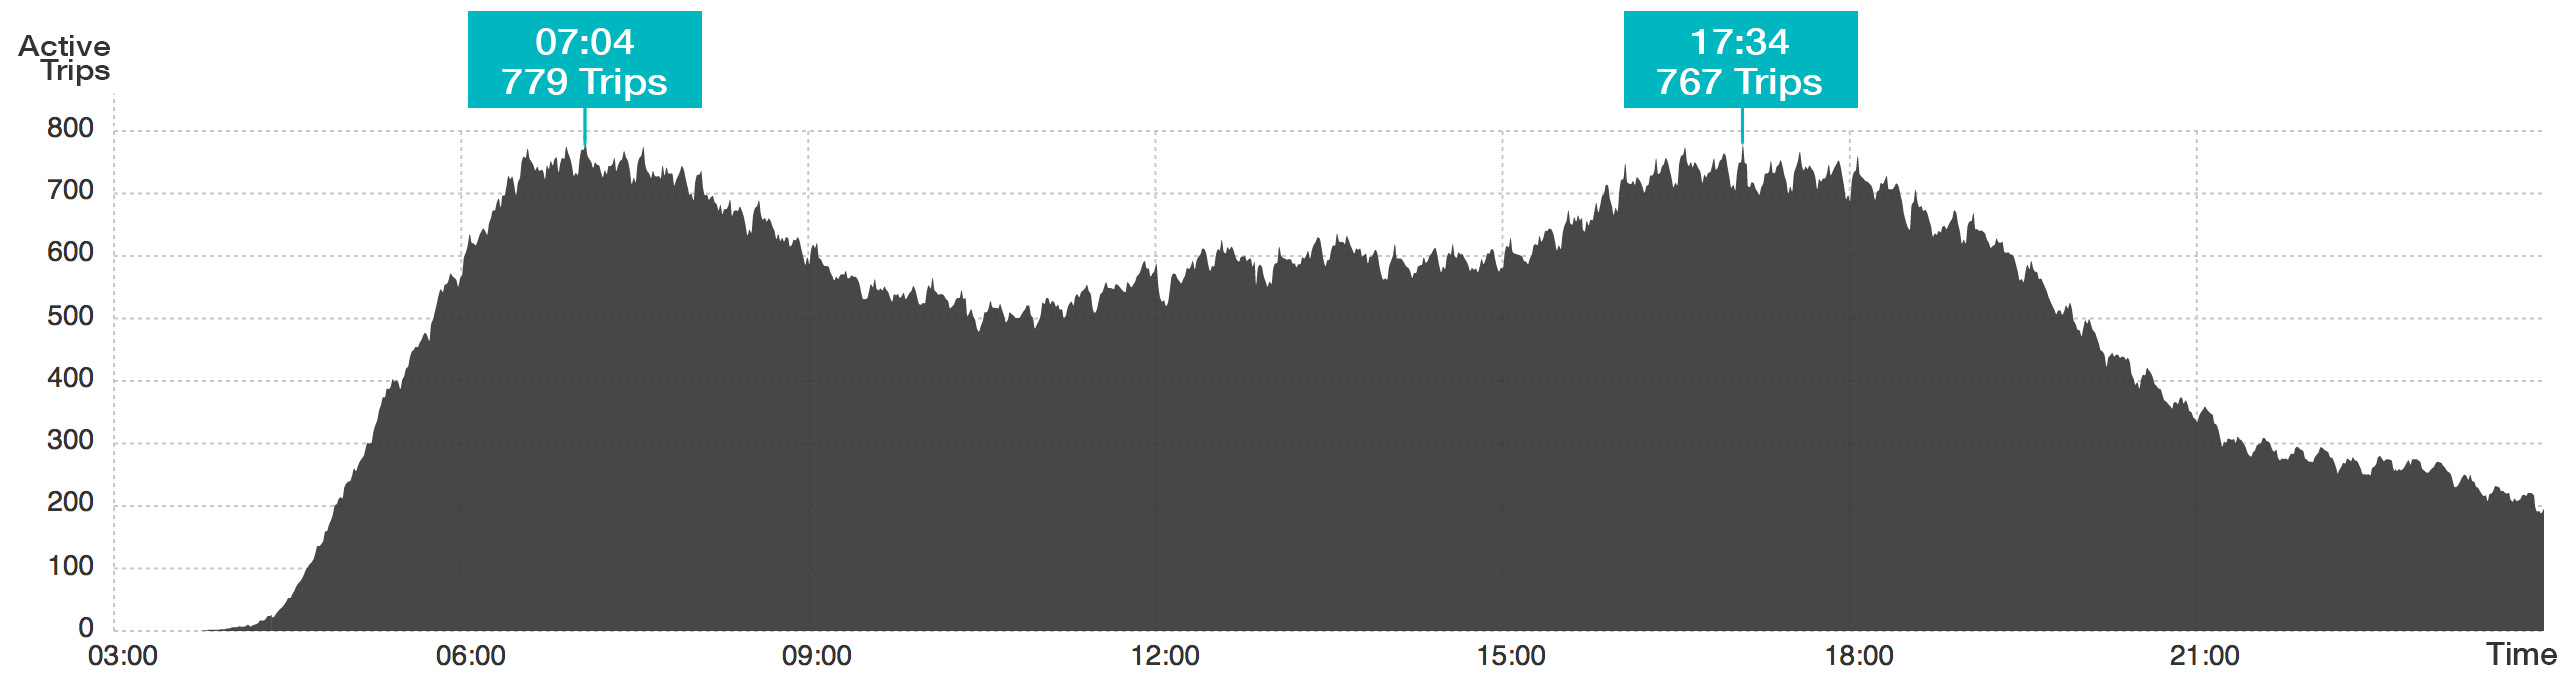
\includegraphics[width=\textwidth]{activeTrips.jpg}
        \caption{Anzahl an aktiven Trips zwischen 3.00 und 24.00 Uhr am 02.08.2017}
        \label{fig:activeTrips}
      \end{center}
    \end{figure}

    Mittags flacht die Anzahl leicht ab, um dann zur Rush Hour am Abend wieder auf 767 gleichzeitig aktive Trips anzusteigen. Anschließend flacht die Anzahl immer weiter ab. Insgesamt wurden an diesem Tag knapp 19650 Trips absolviert. Das Maximum betrug dabei $27 \frac{Trips}{Minute}$ wohingegen das Minimum bei $0 \frac{Trips}{Minute}$ lag. Im Schnitt starten 9 Vehicles pro Minute ihre Fahrt. Für eine interaktive Karte bedeutet dies, dass je nach Tag zwischen 0 und 1000 Trips aktiv sein können. Dies entspricht dann auch der Anzahl an Vehicles die sie auf der Karte bewegen und animiert werden müssen. 
  % subsection bewältigung_der_datenmenge (end)

  \subsubsection{Freiräume in der Gestaltung von GTFS}
  \label{ssub:freiräume_in_der_gestaltung_von_gtfs}
    Trotz der Standardisierung durch GTFS gibt es immer noch diverse Freiräume in der Umsetzung des Formats. Wie anfangs erwähnt wurde, beträgt die Anzahl der Dateien die für ein gültiges GTFS Feed benötigt werden nur 6. Es sind allerdings bis zu 13 Dateien möglich. Dies zeigt wie viele unterschiedliche Informationen ein GTFS Feed bereitstellen kann, aber nicht muss. 
    Auch innerhalb der Dateien gibt es Felder die vorhanden sein "`müssen"' oder nur "`dürfen"'. Beispielsweise muss das Feld \texttt{route\_short\_name} in \texttt{routes.txt} vorhanden sein, aber \texttt{route\_desc} (Route Description) nicht. Der Interpretationsspielraum lässt sich aber noch weiter veranschaulichen, wenn wir uns Tabelle ~\ref{table:gtfs_differences} ansehen. In dieser Tabelle sind Zwei Einträge aus unterschiedlichen GTFS Feeds aufgelistet.
    Wir sehen, dass die Spalte \texttt{route\_id} bei Stuttgart-VVS als Zahlenwert angegeben wird, wohingegen Boston-MBTA einen Text verwendet.

    \begin{longtable}{|>{\raggedright \arraybackslash}p{3.0cm}|>{\raggedright \arraybackslash}p{2.0cm}|>{\raggedright \arraybackslash}p{3.5cm}|>{\raggedright \arraybackslash}p{5.5cm}|}
    \caption{Unterschiede innerhalb GTFS} 
    \label{table:gtfs_differences}\\
      \hline
       & route\_id & route\_short\_name & route\_long\_name\\
      \hline
      Stuttgart-VVS & 379 & U1 & Fellbach - Hauptbahnhof - Vaihingen\\
      \hline
      Boston-MBTA & Blue Line & Blue & Bowdoin - Wonderland\\
      \hline
    \end{longtable}

    "`Blue Line"' ist dabei die Bezeichnung der U-Bahnlinie\parencite{wiki_blue_line}. Wir sehen also, dass Stuttgart-VVS die \texttt{route\_id} zur eindeutigen Identifizierung mittels Zahlenwert verwendet wohingegen Boston-MBTA dieses Feld nutzt, um den Namen der Linie zu beschreiben. Angenommen wir verwenden die \texttt{route\_id} in einer Benutzeroberfläche wie in Abbildung~\ref{fig:gtfs_differences}.

    \begin{figure}[htbp]
      \begin{center}
        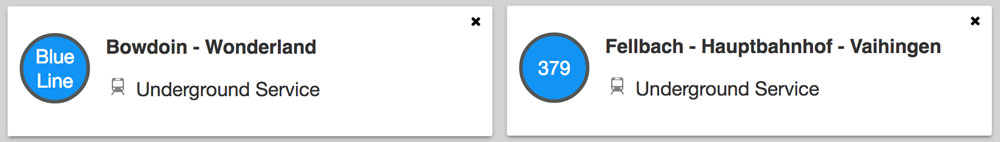
\includegraphics[width=\textwidth]{gtfs_differences.jpg}
        \caption{UI Element mit GTFS Informationen}
        \label{fig:gtfs_differences}
      \end{center}
    \end{figure}

    Links in der Abbildung ist die korrekte Bezeichnung der Route zu sehen nämlich \texttt{Blue Line}, wohingegen rechts nur eine numerische ID zu sehen ist, die nicht für den Nutzer vorgesehen und damit falsch ist. Damit die rechte Seite korrekt wäre müsste dort \texttt{U1} abgebildet sein. Die fehlende beziehungsweise nicht gegebene Übereinstimmung der beiden Feeds führt also zu Problemen bei der Darstellung die auch durch die Verwendung eines anderen Feldes wie zum Beispiel \texttt{route\_short\_name} nicht behoben werden können. 

    Dies ist nur ein Beispiel, bei dem Abweichungen in der Ausführung der Spezifikation eine Auswirkung auf die Programmierung haben. Aus diesem Grund ist im März 2017 auf \url{http://gtfs.org/} eine neue \texttt{Best-Practices} Sektion erschienen. Dabei handelt es sich um Empfehlungen an die Hersteller von GTFS Feeds, um eine Verwendung der Feeds möglichst zu vereinheitlichen. Würden sich alle Hersteller an solch eine striktere Implementierung der Spezifikation halten, müssten Programmierer weniger "`Edge Cases"'\footnotemark abfangen und Anwendungen würden in Qualität und Zuverlässigkeit noch besser werden.\\

    \footnotetext{Ein "`Edge Case"' ist ein Problem oder eine Situation, die nur bei einem extremen (maximalen oder minimalen) Betriebsparameter auftritt.}

    Ein weiteres Problem in GTFS ist das auslesen von Daten. GTFS lässt sich zwar sehr einfach in eine relationale Datenbank überführen, aber das Auslesen der Daten kann schnell sehr komplex werden, sodass die Geschwindigkeit für eine Webanwendung nicht mehr schnell ist. Bereits 1993 stellte \texttt{Jakob Nielsen} einen Richtwert für die responsive Wahrnehmung einer Webanwendung vor:

    \begin{quote}
      \textit{"`1.0 second is about the limit for the user's flow of thought to stay uninterrupted, even though the user will notice the delay. Normally, no special feedback is necessary during delays of more than 0.1 but less than 1.0 second, but the user does lose the feeling of operating directly on the data."'}\parencite{nielsen}
    \end{quote}

    Ob oder wie die Geschwindigkeit erreicht werden kann, soll hier nicht vertieft werden, denn zu diesem Thema habe ich bereits meine Bachelorarbeit gewidmet\parencite{lorer}.

    Damit eine Webanwendung aber überhaupt eine Chance hat, diese Geschwindigkeitsmarke zu erreichen, ist eine schnelle Antwortzeit des Backends sehr wichtig. Dabei sind Antwortzeiten Innerhalb von 1 bis 200 Millisekunden ein sehr guter Wert. Natürlich gilt: Je weniger umso besser. Diese Benchmark mit dem GTFS Format zu erreichen war eine der Hauptherausforderungen dieser Arbeit.\\

    Das GTFS Format hat den entscheidenden Nachteil, dass es eine hohe Komplexität aufweist, sobald Daten aus verschiedenen Tabellen benötigt werden. Für eine Live Visualisierung, sind Daten aus nahezu allen Tabellen relevant. Abbildung \ref{fig:gtfs_joined_tables} zeigt, welche davon benötigt - beziehungsweise nicht benötigt werden (grau).

    \begin{figure}[ht]
      \begin{center}
        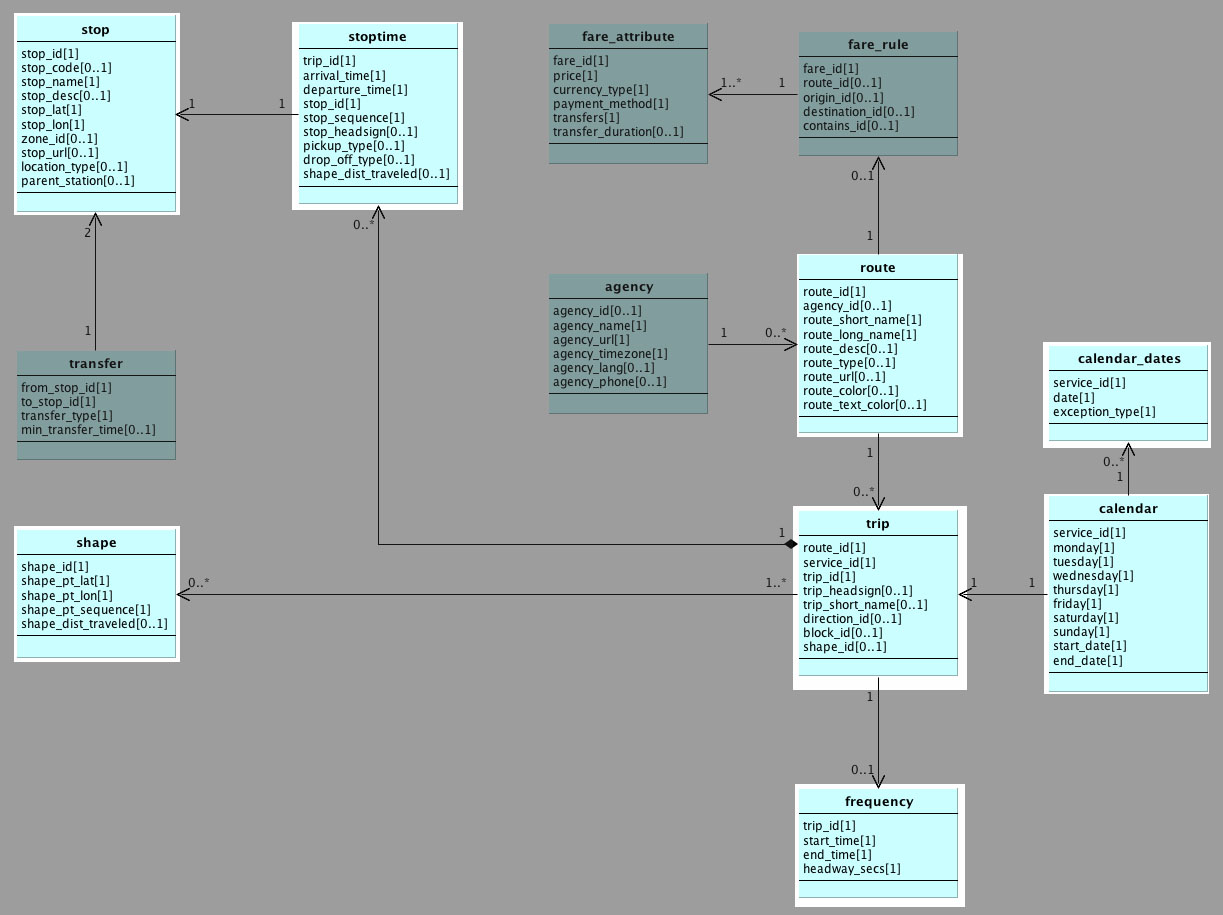
\includegraphics[width=\textwidth]{gtfs_joined_tables.jpg}
        \caption{Benötigte GTFS Tabellen\parencite{google_gtfs_reference}}
        \label{fig:gtfs_joined_tables}
      \end{center}
    \end{figure}

    Das UML Diagramm ist auf den ersten Blick relativ simpel zu verstehen und die Grundlagen der verschiedenen Relationen wurde bereits in Kapitel \ref{ssub:gtfs_fahrplandaten} beschrieben. Wo liegt also das Problem? In Worten ließe sich diese Datenbankabfrage mit folgendem Statement beschreiben: 

    \begin{quote}
      \label{query_statement}
      \textit{"`Gib uns alle aktiven Trips mit deren Linienverlauf, die am heutigen Tag aktiv sind und in einer Zeitspanne zwischen $t_a$ und $t_b$ liegen."'}
    \end{quote}

    Das große Problem dieses Satze liegt in der Zeitkomponente \textit{"`Trips die am heutigen Tag aktiv sind zwischen ..."'}. Die Trip Tabelle selbst (bezogen auf Abbildung \ref{fig:gtfs_joined_tables}), hat dies bezüglich keinerlei Informationen darüber. Auch die Calendar- und Calendar-Dates Tabelle beinhaltet nur Informationen, an welchem Datum ein Trip stattfindet, nicht aber um welche Uhrzeit. 

    Erst die Stoptime Tabelle ermöglicht es uns, eine Aussage zu treffen, wann ein Trip aktiv ist. Über die zwei Felder \texttt{arrival\_time} und \texttt{departure\_time} lässt sich sagen, zu welchem Zeitpunkt ein Vehicle an einer Station anhält. Die erste und letzte Station ($S_1$ und $S_n$) geben uns also einen zeitlichen Rahmen, in dem der Trip aktiv ist.
    Hierbei wird klar, dass allein die Beantwortung der Frage zur zeitlichen Komponente, bereits sehr viele Daten aus verschiedenen Tabellen benötigt. Die anderen Tabellen wie \texttt{shape}, \texttt{route}, \texttt{stop} und \texttt{frequency} würden für weitere Informationen wie Vehicle Farbe, Stop Position (Längen- und Breitengrad) oder die Polyline benötigt werden. Um an die Daten zu gelangen, müssen alle benötigten Tabellen mittels SQL \texttt{JOIN} miteinander verknüpft werden. Dies geschieht durch die Verbindung der einzelnen Reihen zweier Tabellen (TabelleA und TabelleB) gegen eine Verknüpfungsbedingung. Das Resultat ist eine neue Ergebnistabelle mit den Inhalten der kombinierten Reihen. Solche Verknüpfungen sind besonders dann Zeitintensiv, wenn eine große Menge an Daten (siehe Tabelle: \ref{table:table_metrics}) kombiniert werden. Die Metriken der Tabellen sind dabei wie folgt:

    \begin{longtable}{|>{\raggedright \arraybackslash}p{5.0cm}|>{\raggedright \arraybackslash}p{5.0cm}|>{\raggedright \arraybackslash}p{5.0cm}|}
    \caption{Tabellen Metriken} \label{table:table_metrics}\\
      \hline
      Tabellen Name & Anzahl Reihen\\
      \hline
      trips.txt & 71,000\\
      stop\_times.txt & 1,3000,000\\
      stops.txt & 7,900\\
      shapes.txt & 1,085,860\\
      \hline
    \end{longtable}
    
    Die für das oben genannte Statement \ref{query_statement} äquivalente SQL-Abfrage ist aufgrund seiner Länge (113 Zeilen Code) im Anhang unter Listing \ref{lst:get_active_trips_query} zu finden. Diese SQL Abfrage ist allerdings nicht Performant. Sollen alle Trips in einem Zeitraum von 1 - 15 Minuten gefunden werden, sind bereits Rechenzeiten entstanden, die aufgrund ihrer langen Laufzeit abgebrochen werden mussten. In mehreren Iterationen wurde versucht die SQL-Abfrage zu optimieren, was allerdings keine Verbesserung herbeiführte. Es sind zu viele JOIN Verknüpfungen und WHERE Bedingungen in dieser Abfrage, als dass sich eine Performante Lösung damit finden lässt. Es musste ein neuer Ansatz gefunden werden um Abfragezeiten erheblich zu verringern.
  % subsubsection freiräume_in_der_gestaltung_von_gtfs (end)
    
  % section discover (end)
\end{newpage}